\chapter{Algebraic Geometry Codes}\label{chap:alg_geom_codes}
The following chapter is based on \cite{CCC_with_CA}[Section 11.2] and \cite{notes_on_alg_geom_codes}[Chapter 4].
We introduce the codes constructed on curves, we will introduce some new notation. An affine or projective curve $\mathcal{X}$ with defining equation $F = 0$ is said to be a curve over $\mathbb{F}_{q}$ if $F \in \mathbb{F}_{q}[X_1, X_2, \ldots, X_{n}]$ is absolutely irreducible. Furthermore, if $\mathcal{X}$ is an affine or projective curve over $\F_{q}$ then we will let $I(\mathcal{X})$ by the ideal consisting of all polynomials in $\mathbb{F}_{q}[X_1, X_2, \ldots, X_{n}]$ which vanish on $\mathcal{X}$. This ideal is prime both in $\mathbb{F}_{q}[X_1, X_2, \ldots, X_{n}]$ but also in $\cF_{q}[X_1, X_2, \ldots, X_{n}]$, since $F$ being absolutely irreducible implies that $F$ is prime in $\mathbb{F}[X_1, X_2, \ldots, X_{n}]$ and $\cF_{q}[X_1, X_2, \ldots, X_{n}]$. The coordinate ring $\mathbb{F}[\mathcal{X}]$ is defined as $\mathbb{F}_{q}[X_1, X_2, \ldots, X_{n}] / I(\mathcal{X})$, and the function field $\mathbb{F}(\mathcal{X})$ is defined as the quotient field of $\mathbb{F}_{q}[\mathcal{X}]$.\footnote{Notice that it is a subring and field respectively of the usual coordinate ring and function field of $\mathcal{X}$.}

Recall the Frobenius map $\F_{q} \ni x \mapsto x^{q} \in \F_{q}$. The \textit{extended Frobenius map} $\psi$ is simply the Frobenius map extended coordinate wise, to either the $n$ dimensional affine or projective space. We notice that $G(x_1, x_2, \ldots, x_{n})^{q} = G(x_1^{q}, x_2^{q}, \ldots, x_{n}^{q})$ for all $G \in \mathbb{F}_{q}[X_1, X_2, \ldots, X_{n}]$ and $x_1, x_2, \ldots, x_{n} \in \mathbb{F}_{q}$ by freshman's dream. Hence, if $\mathcal{X}$ is an affine or projective curve defined over $\F_{q}$ then $P \in \mathcal{X}$, implies $\psi(P) \in \mathcal{X}$.

A divisor $D \in Div(\mathcal{X})$ is called rational if the weight of $P$ and $\psi(P)$ is the same for all $P \in \mathcal{X}$. The vector space $L(D)$ will only consist of rational divisors and is otherwise defined as before, albeit with the restriction of the rational functions to $\mathbb{F}_{q}(\mathcal{X})$. However, even with these changes the Reimann Roch Theorem \ref{thm:reimann_roch} remains true, confer both of the sources listed earlier.

Finally, let $\mathcal{P} := (P_1, P_2, \ldots, P_{m})$ be a tuple of points, then we define the \textit{evaluation map} as in Example \ref{exmp:rs_codes} to be the map as $\ev(F) = (F(P_1), F(P_2), \ldots, F(P_{m}))$. The domain of $\ev$ will either be a subset of $\F_{q}(\mathcal{X}) \setminus \left\{0\right\}$ or $\F_{q}[X_1, X_2, \ldots, X_{n}]$.
\newpage
\section{Codes Constructed on Affine Plane Curves}
We will start by considering codes constructed from affine plane curves, as this is the simplest case to understand. Our proof of the following proposition will be based on the proof of \cite{CCC_with_CA}[Proposition 11.2.1].
\begin{proposition}\label{prop:plane_code}
  Let $F$ be an absolutely irreducible polynomial in $\mathbb{F}_{q}[X, Y]$, of degree $m$, and let $\mathcal{X}$ be the curve with defining equation $F = 0$. Furthermore let $P_1, P_2, \ldots, P_{n} \in \mathcal{X}$ be $n$ distinct rational points and $\mathcal{P} := (P_1, P_2, \ldots, P_{n})$. Finally consider the linear code:
  \begin{equation*}
    E(l) = \left\{\ev(G) \mid G \in \mathbb{F}_{q}[X, Y], \deg(G) \leq l\right\}.
  \end{equation*}
  Then if $lm < n$, then the minimum distance $d$ and dimension $k$ of $E(l)$ satisfies:
  \begin{align*}
    d &\geq n  - lm \\
    k &= \begin{cases} \binom{l + 2}{2} & \text{ if } l < m \\
                      lm  + 1 - \binom{m - 1}{2} & \text{ otherwise }
        \end{cases}
  \end{align*}
\end{proposition}
\begin{proof}
  Let $V_{l} \subseteq \mathbb{F}_{q}[X, Y]$ be the $\mathbb{F}_{q}$ vector space of polynomials with degree at most $l$, notice that $\ev(V_{l}) = E(l)$. Then the monomials $X^{i}Y^{j}$, with $i + j = 0, 1, \ldots, l$ form a basis of $V_{l}$. Since there is $\binom{l + 2}{2}$ of these the vector space $V_{l}$ has dimension $\binom{l + 2}{2}$. \\
  Let $G \in V_{l}$, if $F$ factors $G$, then $\ev(G) = 0$. Conversely, if $\ev(G) = 0$, then the projective curves with defining equations $F^{*} = 0$ and $G^{*} = 0$, have degrees $\deg(G) \leq l$ and $m$ respectively but intersect at $n$ points namely $\phi(P_{1}), \phi(P_{2}), \ldots, \phi(P_{n})$, where $\phi(x_1, x_2, \ldots, x_{n}) = [x_1: x_2 : \cdots :  x_{n} : 1]$. This is a contradiction since $\deg(G)m \leq lm < n$ and Bézout's Theorem \ref{thm:bézouts} implies that they intersect in at most $\deg(G)m$ points. Hence $F$ and $G$ must have a common factor; meaning $G$ is divisible by $F$ as $F$ is irreducible. Hence, $\ev$ restricted to $V_{l}$ have kernel $FV_{l - m}$. Now if $l < m$, then $FV_{l - m}$ has dimension $0$ and hence:
  \begin{equation*}
    k = \dim_{\mathbb{F}_{q}}(E(l)) = \dim_{\mathbb{F}_{q}}(V_l) - \dim_{\mathbb{F}_{q}}(FV_{l - m}) = \binom{l + 2}{2}
  \end{equation*}
  since $\ev$ is a linear map. Conversely if $l \geq m$ we obtain:
  \begin{align*}
    k = \binom{l + 2}{2} - \binom{l - m + 2}{2} = \frac{-m^{2} - 2lm + 3m}{2} = lm + 1 - \binom{m - 1}{2}
  \end{align*}
  Finally by a similar argument as earlier, by Bézouts Theorem \ref{thm:bézouts} a nonzero codeword has at most $lm$ zeros. Hence the minimum weight of $E(l)$ is at least $n - lm$.
\end{proof}

The results of Proposition \ref{prop:plane_code} indicate that if we want $E(l)$ to have a high minimum distance, we should choose $F$ and $l$ such that $\deg(F)$ and $l$ are as small as possible, while maximizing the number of rational points on $\mathcal{X}$. \\
Conversely if we want to maximize the dimension of $E(l)$ then we should choose $F$ and $l$ such that $\deg(F)$ and $l$ are as large as possible, albeit such that $l\deg(F)$ is strictly less than the number of rational points on $\mathcal{X}$.

\begin{example}\label{exmp:code_from_plane_curve_rs}
  If we pick $F = Y - 1$ and let $\mathcal{X}$ be the affine plane curve with defining equation $F = 0$. Then the set of rational points of $\mathcal{X}$ consist of the points $P = (a, 1)$ where $a \in \F_{q}$. Let $G \in \F_{q}[X, Y]$ such that $\deg(G) \leq l$ then $G(X, 1)$ is an univariate polynomial of degree less than or equal to $l$. Hence the linear code $E(l)$, where $l \in \N$, corresponds to the Reed-Solomon code of degree $l + 1$.
\end{example}

\newpage
\section{Goppa Codes}\label{sec:goppa_codes}
In this section we will introduce codes on constructed projective algebraic curves (not necessarily in the protective plane) and show some results on the parameters of these.

\begin{definition}
  Let $\mathcal{X}$ be an absolutely irreducible regular projective curve over $\mathbb{F}_{q}$ and $P_1, P_2, \ldots, P_{n} \in \mathcal{X}$ be $n$ distinct rational points. Let $D = \sum_{i = 1}^{n} P_{i}$ and $G \in Div(\mathcal{X})$ such that $\support(D) \cap \support(G) = \emptyset$, then the linear code $C_{D, G} := \ev(L(G))$, where $\mathcal{P} := (P_1, P_2, \ldots, P_{n})$, is called an \textit{algebraic geometry code} or
  a \textit{Goppa code}.
\end{definition}
As noted in Section \ref{sec:bounds}, the family of Reed-Solomon codes (see Example \ref{exmp:rs_codes}), are a subfamily of the family of algebraic geometry codes. We will show this in the following example which is based on \cite{notes_on_alg_geom_codes}[Exercise 4.2].
%\begin{example}\label{exmp:rs_is_goppa}
%  We will show that these codes are Goppa codes constructed from the curve $\mathcal{X}$ with defining equation $Y = 0$ and divisors $D = \sum_{i = 1}^{n}P_{i}$ and $G = (k - 1)P_{\infty}$ where $1 \leq k \leq n \leq q$, $P_{i} = [i : 0 : 1]$ and $P_{\infty} = [1 : 0 : 0]$. From Example \ref{exmp:divisors_for_rs_codes} we have that:
%  \begin{equation*}
%    L(G) = \left\{F(X, Z) / Z^{k -1} \mid F(X, Y) \in \cF_{q}[X, Z], \text{ homogeneous with } \deg(F) \leq k - 1\right\}
%  \end{equation*}
%  Hence if $f = \frac{F(X, Z)}{Z^{k - 1}} \in L(G)$, then $f(P_{i}) = \frac{F(i, 1)}{1^{k - 1}} = F(i)$ for $i = 1, 2, \ldots, n$, as $F$ and $Z^{k - 1}$ are homogeneous polynomials.
%  Thus given a codeword $c = (f(P_1), f(P_2), \ldots, f(P_{n})) \in C_{D, G}$, where $f = F(X, Z) / Z^{k - 1} \in L(G)$ then $c = (F(1, 1), F(2, 1), \ldots, F(n, 1))$, this is a codeword in the Reed-Solomon code of degree $k$, since $\deg(F) \leq k - 1$.
%\end{example}

\begin{example}\label{exmp:rs_is_goppa}
  Let $1 \leq k \leq n \leq q$, let $\mathcal{X}$ be the projective plane curve with defining equation $Y = 0$ and divisors $D = \sum_{i = 1}^{n}P_{i}$ and $G = (k - 1)P_{\infty}$ where $P_{i} = [i : 0 : 1]$ and $P_{\infty} = [1 : 0 : 0]$. From Example \ref{exmp:divisors_for_rs_codes} we have that:
  \begin{equation*}
    L(G) = \left\{F(X, Z) / Z^{k -1} \mid F(X, Y) \in \cF_{q}[X, Z], \text{ homogeneous with } \deg(F) \leq k - 1\right\}
  \end{equation*}
  Consider the codeword $c = (f(P_{1}), f(P_2), \ldots, f(P_{n})) \in \mathcal{C}_{D, G}$, where $f(X, Y, Z) = \frac{F(X, Z)}{Z^{k - 1}}$, such that $\deg(F) \leq k - 1$ and $F$ is homogeneous, then $f \in L(G)$. Then writing $F = \sum_{i = 0}^{\deg(F)} a_{i}X^{i} Z^{\deg(F) - i}$ and letting $F_{*}(X) := F(X, 1) = \sum_{i = 0}^{\deg(F)} a_{i} X^{i}$ we see that $c$ equal to the codeword $(F_{*}(1), F_{*}(2), \ldots, F_{*}(n))$ of the Reed-Solomon code of degree $k$, since $\deg(F) \leq k - 1$.
\end{example}

Clearly since every Reed-Solomon code is a MDS code, Goppa codes with good parameters can be constructed. One of the advantages of Goppa codes is that we can obtain good lower bounds for their minimum distance, this is along with other things what we will show in the following theorem:
\begin{theorem}\label{thm:goppa_code_properties}
  Let $C_{D, G}$ be a $[n, k, d]_{q}$ code. Then
  \begin{enumerate}
    \item $k = \ell(G) - \ell(G - D)$. \label{thm:goppa_code_property:1}
    \item $d \geq n - \deg(G)$. \label{thm:goppa_code_property:2}
  \end{enumerate}
\end{theorem}
\begin{proof}
  We start by proving Assertion \ref{thm:goppa_code_property:1}. The map $\ev$ is a surjective linear map from $L(G)$ to $C_{G, D}$. Hence,
  \begin{equation*}
    k = \dim_{\mathbb{F}_{q}}(\image(\ev)) = \ell(G) - \dim_{\mathbb{F}_{q}}(\ker(\ev)) = \ell(G) - \ell(G - D)
  \end{equation*}
  where the last equality follows as $\ker(\ev) = L(G - D)$. This equality can be seen as follows: If $f \in L(G)$ and $\ev(f) = 0$, then $v_{P_{i}}(f) \geq 1$ for all $i = 1, 2, \ldots, n$, and hence $(f) + G - D$ is effective meaning $f \in L(G - D)$, conversely if $f \in L(G - D)$, then $f$ vanishes at every $P \in \support(D)$ as $\support(G) \cap \support(D) = \emptyset$. This means that $f \in \ker(\ev)$.

  Continuing with Assertion \ref{thm:goppa_code_property:2}. Suppose $c \in \mathcal{C}_{G, D}$ then there exists $f \in \mathbb{F}_{q}(\mathcal{X})$ such that $c = (f(P_1), f(P_2), \ldots, f(P_{n}))$. Assuming $\wt(c) = d$, then $f$ vanishes at $n - d$ points, say $P_{i_{1}}, P_{i_{2}}, \ldots, P_{i_{n - d}}$. This in turn implies that $f \in L\left(G - \sum_{j = 1}^{n- d} P_{i_{j}}\right)$ as $G - \sum_{j = 1}^{n - d} P_{i_{j}} + (f)$ are effective because $v_{P_{i_{j}}}(f) \geq 1$ for all $j = 1, 2, \ldots, n - d$. Hence,
  \begin{equation*}
    \deg \left(G - \sum_{j = 1}^{n - d} P_{i_{j}}\right) \leq \deg((f)) = 0
  \end{equation*}
  by Proposition \ref{prop:principal_divisors_are_well_defined}. However, as $\deg \left(G - \sum_{j = 1}^{n - d} P_{i_{j}}\right) = \deg(G) - n + d$ this yields the desired result.
\end{proof}

Imposing extra conditions on the degree of $G$ yields further results on the dimension of $\mathcal{C}_{D, G}$, these results are stated and proved in the following corollary.

\begin{corollary}\label{cor:goppa_code_properties2}
  Suppose $\mathcal{X}$ be an absolutely irreducible regular projective curve over $\mathbb{F}_{q}$ of genus $g$. Let $\mathcal{C}_{D, G}$ be a $[n, k, d]_{q}$ Goppa code on $\mathcal{X}$. Then the following assertions hold:
  \begin{enumerate}
    \item If $\deg(G) < n$, then $k = \ell(G)$. Furthermore if $f_1, f_2, \ldots, f_{k}$ is an $\mathbb{F}_{q}$-basis of $L(G)$, then a generator matrix of $\mathcal{C}_{G, D}$ is given by:
          \begin{equation*}
            M := \begin{bmatrix}
                   f_{1}(P_{1}) & f_{1}(P_{2}) & \cdots & f_{1}(P_{n}) \\
                   f_{2}(P_{1}) & f_{2}(P_{2}) & \cdots & f_{2}(P_{n}) \\
                  \vdots & \vdots & \ddots & \vdots \\
                   f_{k}(P_{1}) & f_{k}(P_{2}) & \cdots & f_{k}(P_{n})
                 \end{bmatrix}
        \end{equation*} \label{cor:goppa_codes_properties2:1}
      \item If $2g - 2 < \deg(G) < n$, then $k = \deg(G) - g + 1$. \label{cor:goppa_code_properties2:2}
  \end{enumerate}
\end{corollary}
\begin{proof}
  We start by proving the first claim of Assertion \ref{cor:goppa_codes_properties2:1}. Notice that $\deg(G - D) = \deg(G) - \deg(D) < n - n = 0$ implies that $\ell(G - D) = 0$ by Proposition \ref{prop:dimension_of_vector_space_of_divisors}. \\ Next we show that $M$ is a generator matrix of $\mathcal{C}_{D, G}$. It is sufficient to show that the rows $m_1, m_2, \ldots, m_{k}$ of $M$ are $\mathbb{F}_{q}$-linearly independent since all $k$ of them are codewords. Suppose $\sum_{i  = 1}^{k} a_{i} m_{i} = 0^{T}$ with $a_1, a_2, \ldots, a_{k} \in \mathbb{F}_{q}$, then $\sum_{i = 1}^{k} a_{i} f_{i}(P_{j}) = 0$ for $j = 1, 2, \ldots, n$. Letting $g := \sum_{i = 1}^{k} a_i f_{i}$ we see that $g$ vanishes at $P_1, P_2, \ldots, P_{n}$ and hence $g \in L(G - D) = \left\{0\right\}$, meaning $a_{1} = a_{2} = \cdots = a_{k} = 0$.

  Assertion \ref{cor:goppa_code_properties2:2}, follows from Assertion \ref{thm:goppa_code_property:1} as $k = \ell(G)$, when $\deg(D) < n$. This along with the fact that $2g - 2 < \deg(G)$ imply that $\ell(G) = \deg(D) - g + 1$ by Corollary \ref{cor:degree_less_than_2g-2}, yielding the desired result.
\end{proof}

\begin{remark}\label{rem:goppa_codes_MDS}
  Assertion \ref{cor:goppa_codes_properties2:1} of Corollary \ref{cor:goppa_code_properties2}, says that $k = \ell(G)$, combining this with the Reimann Roch Theorem \ref{thm:reimann_roch} we see that $k = \ell(G) \geq \deg(G) - g + 1$, combining this with Assertion \ref{thm:goppa_code_property:1} of Theorem \ref{thm:goppa_code_properties}, we see that $d + k \geq (n - \deg(G)) + (\deg(G) - g + 1) = n - g + 1$.
  Recall that the Singleton Bound, Corollary \ref{cor:singleton_bound}, states that every $[n, k, d]_{q}$ code satisfies $d - 1 \leq n - k$. Combining these facts we see that: $n - g + 1 \leq d + k \leq n + 1$ and in particular if $\mathcal{C}_{D, G}$ is constructed on a curve of genus $0$, then $\mathcal{C}_{D, G}$ is a MDS code.
\end{remark}

\newpage
\subsection{Constructing Good Goppa Codes}

Let $\mathcal{X}$ be a projective curve and $C_{D, G}$ be a Goppa code constructed on $\mathcal{X}$. If $C_{D, G}$ is a $[n, k, d]_{q}$ code, then $k + d \geq n - g + 1$ by Remark \ref{rem:goppa_codes_MDS}. If we divide by $n$ we see that the transmission rate $R$ and relative minimum distance $\delta$ of $C_{D, G}$ satisfy the following inequality:
\begin{equation}\label{eq:R_and_delta_of_goppa}
  R + \delta  \geq 1 - \frac{g - 1}{n}.
\end{equation}
Hence in order to construct Goppa codes with good parameters, we need to maximize the ratio $N_{q}(\mathcal{X}) / g(\mathcal{X})$, where $N_q(\mathcal{X})$ is the number of rational points on $\mathcal{X}$ and $g(\mathcal{X})$ is the genus of $\mathcal{X}$.

We state the following result, which where proved by Tsfasman Vlăduţ and Zink without proof.
\begin{theorem}\label{thm:bound_on_ratio}
  Let $q = p^{2}$ where $p$ is a prime. Let $N_{q}^{*}(g)$ be the maximum number of $\F_{q}$-rational points on an absolutely irreducible smooth projective curve over $\F_{q}$ with a genus less than or equal to $g$. Then:
  \begin{equation*}
    \underset{g \to \infty}{\lim \sup}\;\frac{N_{q}^{*}(g)}{g} \leq \sqrt{q} - 1.
  \end{equation*}
\end{theorem}
Theorem \ref{thm:bound_on_ratio} implies the existence of a sequence $\left\{\mathcal{X}_{g}\right\}_{g \in \N}$ of smooth projective curves over $\F_{q}$, where $\mathcal{X}_g$ has genus $g$, such that $\underset{g \to \infty}{\lim \sup}\; \frac{N_{q}(\mathcal{X}_{g})}{g} \leq \sqrt{q} - 1$, and hence $\underset{g \to \infty}{\lim \sup}\; \frac{g}{N_{q}(\mathcal{X}_{g})} \geq \frac{1}{\sqrt{q} - 1}$. Combining this with equation \eqref{eq:R_and_delta_of_goppa} we see that there exists a sequence of Goppa codes $\left\{\mathcal{C}_{D_{g}, G_{g}}\right\}_{g \in \N}$ where $\mathcal{C}_{D_g, G_g}$ is constructed on $\mathcal{X}_g$ such that:
\begin{equation}\label{eq:TVZ_bound}
  \underset{g \to \infty}{\lim \sup} \; R(\mathcal{C}_{D_g, G_g}) + \delta(\mathcal{C}_{D_g, G_g}) \geq 1 - \frac{1}{\sqrt{q} - 1}
\end{equation}
The inequality in equation \eqref{eq:TVZ_bound} is called the \textit{Tsfasman–Vlăduţ–Zink bound}. If $q \geq 49$, then this bound exceeds the asymptotic Gilbert-Varshaomov bound, meaning $1 - \frac{1}{\sqrt{q} - 1} > 1 - H_{q}(\delta) + \delta$ albeit only in a certain range of transmission rates / relative minimum distances, see Figure \ref{fig:tvz}.
However since $R = k / n$ we can construct Goppa codes with parameters in this range, confer Assertion \ref{cor:goppa_code_properties2:2} of Corollary \ref{cor:goppa_code_properties2}.
\begin{figure}[H]
    \centering
    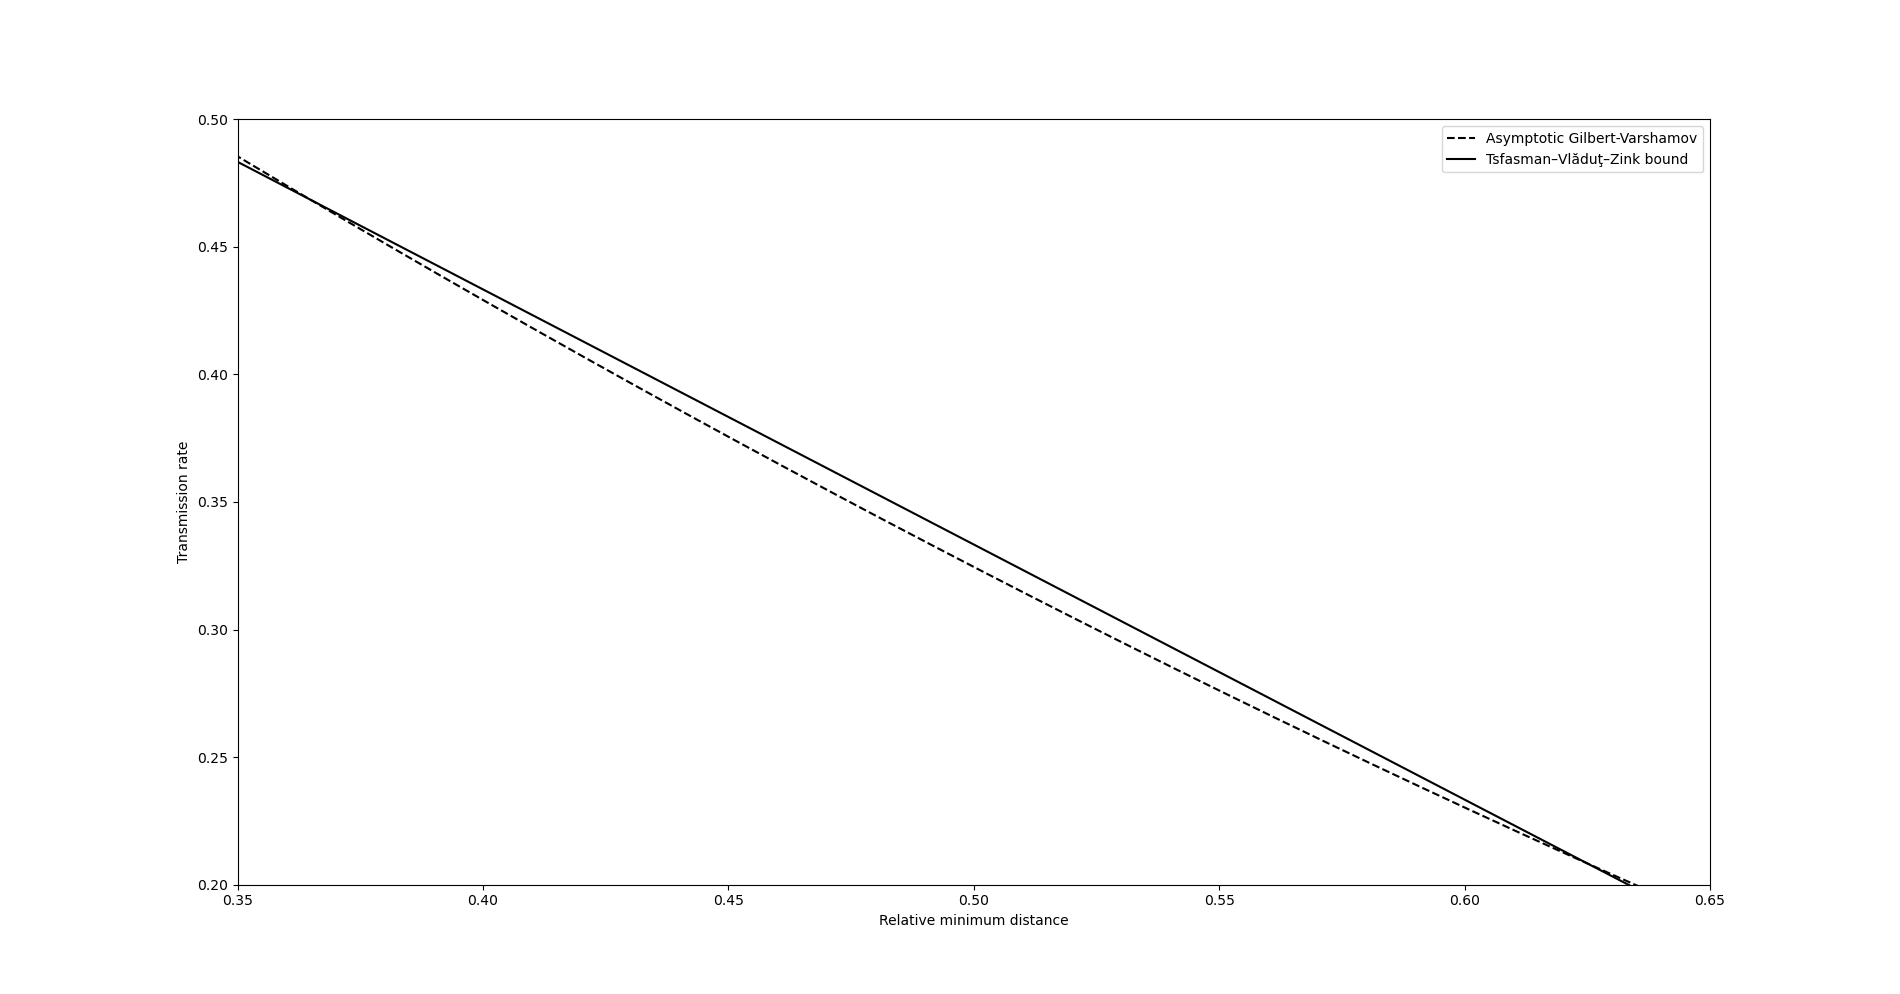
\includegraphics[trim={3cm 1cm 3cm 2cm},clip, scale=0.35]{tvz.png}
    \caption{The Asymtotic Gilbert-Varshamov bound versus the Tsfasman–Vlăduţ–Zink bound for $q = 49$.}
    \label{fig:tvz}
\end{figure}
The fact that one is able to construct sequences of Goppa codes with parameters that exceed the asymptotic Gilbert-Varshamov bound, was in fact one of the reasons for the initial interest in algebraic geometry codes.
%\subsection{The Tsfasman–Vlăduţ–Zink bound}
%However upper bounds on the number of rational points of a projective curve do exist, we state the following without proof.
%\begin{theorem}[Hasse-Weil bound]\label{thm:hasse_weil_bound}
%  Let $\mathcal{X}$ be a smooth projective curve over $\F_{q}$ of genus $g$. Let $N_{q}(\mathcal{X})$ denote the number of $\mathbb{F}_{q}$-rational points of $\mathcal{X}$. Then
%  \begin{equation*}
%    \abs{N_{q}(\mathcal{X}) - (q + 1)} \leq g \lfloor 2\sqrt{q}\rfloor
%  \end{equation*}
%\end{theorem}

